\documentclass{article}

\usepackage{amsfonts}
\usepackage{amsmath}
\usepackage{tikz}

\begin{document}
\begin{table}
\centering
\caption{Versions}
\begin{tabular}{|l|l|}
\hline
Date & Summary\\
\hline
2015-12-10 & Initial version.\\
2016-5-2 & Corrected port image for 6mm Pitot. \\
\hline
\end{tabular}
\end{table}


\begin{figure}
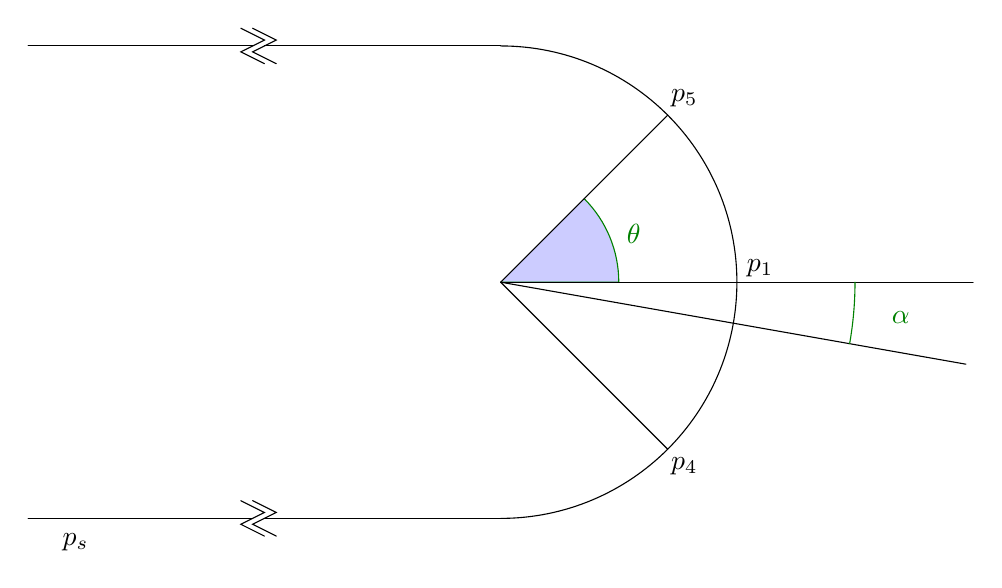
\begin{tikzpicture}[scale=3,cap=round]
  % Local definitions
  \def\costhirty{0.8660256}

  % Colors
  \colorlet{anglecolor}{green!50!black}
  \colorlet{sincolor}{red}
  \colorlet{tancolor}{orange!80!black}
  \colorlet{coscolor}{blue}

  % Styles
  \tikzstyle{axes}=[]
  \tikzstyle{important line}=[very thick]
  \tikzstyle{information text}=[rounded corners,fill=red!10,inner sep=1ex]



  %\draw (0,0) circle (1cm);
  \draw (1,0) arc (0:90:1cm);
  \draw (1,0) arc (0:-90:1cm);

  \draw (0,1) -- (-1.0,1);
  \draw (-1.05,1) -- (-2,1);
  \draw (-1.05, 1.075) -- (-0.95, 1.025) -- (-1.05, 0.975) -- (-0.95, 0.925);
  \draw (-1.1, 1.075) -- (-1.0, 1.025) -- (-1.1, 0.975) -- (-1.0, 0.925);

  \draw (0,-1) -- (-1.0,-1);
  \draw (-1.05,-1) -- (-2,-1);
  \draw (-1.05,-0.925 ) -- (-0.95, -0.975) -- (-1.05, -1.025) -- (-0.95, -1.075);
  \draw (-1.1, -0.925) -- (-1.0, -0.975) -- (-1.1, -1.025) -- (-1.0, -1.075);

  %\begin{scope}[style=axes]
  %  \draw[->] (-1.5,0) -- (1.5,0) node[right] {$x$};
  %  \draw[->] (0,-1.5) -- (0,1.5) node[above] {$y$};
  %\end{scope}

  \filldraw[fill=blue!20,draw=anglecolor] (0,0) -- (5mm,0pt) arc(0:45:5mm);
  %\filldraw[fill=blue!20,draw=anglecolor] (0,0) -- (5mm,0pt) arc(0:-45:5mm);
  \draw (20:6mm) node[anglecolor] {$\theta$};
  \draw (0,0) -- (45:1cm);
  \draw (45:1.1cm) node {$p_5$};
  \draw (0,0) -- (-45:1cm);
  \draw (-45:1.1cm) node {$p_4$};
  \draw (3:1.1cm) node {$p_1$};
  \draw (-1.8, -1.1) node {$p_s$};
  \draw (0,0) -- (2cm,0);
  \draw (0,0) -- (-10:20mm);
  \draw[draw=anglecolor] (15mm,0pt) arc(0:-10:15mm);
  \draw (-5:17mm) node[anglecolor] {$\alpha$};
\end{tikzpicture}
\caption{Sketch of 5 port pitot tube angle-of-attack sensing ports and
  flow direction.\label{fig:pitot}}
\end{figure}
\begin{figure}
\centering
\includegraphics[width=0.4\textwidth]{pitot_ports.png}
\caption{Port layout at Aeroprobe pitot tip with port numbering.}
\end{figure}


\section{Pitot Sensing Airspeed and Angle-of-Attack}

\subsection{Importance of Low-Speed Flight for first Trans-In}
There are two needs for low-speed angle-of-attack sensing during early
trans-in flights.  The first is during the powered climb phase of
trans-in for stall-prevention.  The main-wing is predicted to stall at
approximately 6$^\circ$ angle-of-attack.  There is a stall hysterisis
of approximately 4$^\circ$.  For this reason, we plan to fly below
$2^\circ$ angle-of-attack.  Sensing error will drive how close we can
comfortably fly to this limit, which in turn drives our achievable
lift, and whether or not we successfully trans-in.

A second driver is low-speed high-angle of attack sensing during the
initial pitch forward.  If we have an airspeed of $10$ m/s, and there
is an updraft of $5$ m/s, up to $20-30^\circ$ of angle-of attack error
can be induced compared to assuming wind lies in the plane.  For this
range it is only important that the growth in error is slower than the
growth in angle of attack so that the controller knows to continue to
pitch forward.  An example of such an envelope would be to require a
maximum of $1.5^\circ$ of total error for true angles less than
$6^\circ$ and at most $0.1$ deg/deg growth in error for higher angles.

\subsection{Measuring Angle-of-attack with a 5-Port Pitot}
There are many sources of error in measuring angle of attack with a
5-port pitot tube.  Here is a list of factors an ways we can mitigate them:

\begin{description}
\item[Local airflow:] Careful placement via CFD.
\item[Mechanical alignment:]
\item[Tube geometry:] Require vendor calibration at relevant airspeeds.
\item[Air density variation:] Sense outside-air-temperature, protect for humidity.
\item[Pressure sensor errors:] Discussed in this document.
\item[Compressibility:] Concern for higher speed flight.
\end{description}

\subsection{Effects of Pressure Sensor Errors}
We model the hemispherical end of the pitot tube as a sphere (see
equaiton 2.7 on page 6 of \cite{mhp}).  The inviscid, incompressible
pressure distribution over a sphere is given by:
\begin{equation}
C_P = \frac{p - p_\infty}{q_\infty} = 1 - \frac{9}4 \sin(\gamma)^2,
\end{equation}
where $\gamma$ is the angle between the stagnation point and the point
of interest.  Given the port layout on the Aeroprobe 5-port Pitot tube
tip the differential pressures we measure would be given by:
\begin{equation}
p_q = p_1 - p_s = q_\infty \left(1 - \frac{9}4 \left(\sin(\alpha)^2\cos(\beta)^2
+ \sin(\beta)^2\right)\right).
\end{equation}
\begin{equation}
p_\alpha = p_4 - p_5 = \frac{9}4 q_\infty \sin(2\theta)\cos(\beta)^2\sin(2\alpha),
\end{equation}
\begin{equation}
p_\beta = p_3 - p_2 = \frac{9}4 q_\infty \sin(2\theta)\cos(\alpha)\sin(2\beta),
\end{equation}
where the angle of attack is measured as in Figure~\ref{fig:pitot}.
Best sensitivity is given by taking $\theta = \frac{\pi}{4}$, which appears to be
the case on the Aeroprobe pitot tubes we plan to use.
The differential pressure between the dynamic and static ports is given by:
The measured differential pressure ($\tilde p_\alpha$) and dynamic
pressure ($\tilde q_\infty$) will have errors:
\[
\tilde p_\alpha = p_\alpha + \delta_{p_{\alpha}}, \quad \tilde
p_q = p_q + \delta_{p_q}.
\]



%% A linearized analysis gives the sensitivity of the unknowns
%% ($q_\infty$ and $\alpha$) as a function of small pressure errors:
%% \begin{equation}
%% \begin{bmatrix}
%% \delta_\alpha \\
%% \delta_{q_\infty}
%% \end{bmatrix}
%% =
%% \begin{bmatrix}
%% \frac{9}2 q_\infty \cos(2\alpha) &
%% \frac{9}4  \sin(2\alpha)
%% \\
%% -\frac{9}4 q_\infty \sin(2\alpha) &
%% 1 - \frac{9}4 \sin(\alpha)^2
%% \end{bmatrix}^{-1}
%% \begin{bmatrix}
%% \delta_{p_\alpha} \\
%% \delta_{p_d}
%% \end{bmatrix}
%% \end{equation}

\subsection{Part selection for Honywell HSC Series sensors}
The Honeywell HSC series pressure sensors that we are using report
their errors in terms of two percentages against full-scale-span
(FSS).  For a differential pressure sensor, measuring between $\pm 1$
kPa the FSS is $2$ kPa (see footnote 8 under stable 5 on page 9 in
\cite{Honeywell}).  Two measures of error are given (see also Figure~\ref{fig:accuracy}):
\begin{description}
\item[Accuracy] This is decribed as a percent of the FSS that the
  sensor deviates from the best-fit-straight-line (BFSL).  It accounts
  for pressure non-linearity, hystersis and non-repeatability, but not
  thermal effects on these quantities.
\item[Total Error Band] This is a percent FSS which covers operation
over the entire range of calibrated temperatures.
\end{description}
\begin{figure}
\centering
\includegraphics[width=\textwidth]{honeywell.png}
\caption{Error description from \cite{Honeywell}\label{fig:accuracy}.}
\end{figure}
From a first reading of the datasheet, we need to perform a
per-temperature calibration of the BFSL ourselves to achieve the
accuracy numbers.  It is unclear if there is hysterisis when
performing temperature cycles.

Based on the simple pressure model of the previous section, we can
plot the sensitivity of angle-of-attack and airspeed to pressure
sensing errors see Figure~\ref{fig:sensitivity}.  We use $\rho = 1.02$
kg/m$^3$ as a worst case operating point.
\begin{figure}
\centering
\includegraphics[width=\textwidth]{sensitivity.png}
\caption{Sensitivity of angle-of-attack ($\alpha$) and airspeed
  $V_\infty$ measurements to pressure sensing errors as varying
  airspeed.  We assume an air-density of 1.02 kg/m$^3$. \label{fig:sensitivity}}
\end{figure}
Tables~\ref{hsc_errors} and~\ref{hsc_airspeed_errors} list the effect
of pressure errors for two sensing ranges.  These errors are evaluated
by solving for estimates of $\alpha$ and $V_\infty$ with the corner
points of measured pressures ranges and looking at the worst case
error.

\begin{table}
\caption{Angle-of-Attack Errors at $\beta = 0^\circ, \alpha = 6^\circ$ from Pressure Sensor Errors \label{hsc_errors}}
\begin{tabular}{|l|l|l|l|}
\hline
Presure Range & $V_\infty$ [m/s] & $\alpha$ Error ($\pm 0.25\%$ FSS) & $\alpha$ Error ($\pm 1\%$ FSS) \\
\hline
$\pm 1$ PSI & 15 & 7.1 & X \\
 & 20 & 3.54 & 22 \\
 & 40 & 0.8 & 3.5 \\
$\pm 600$ Pa & 15 & 0.5 & 2.1 \\
& 20 & 0.27 & 1.13 \\
& 40 & 0.07 & 0.27\\
\hline
\end{tabular}
\end{table}
\begin{table}
\caption{Airspeed Errors at $\beta = 0^\circ, \alpha = 6^\circ$ from Pressure Sensor Errors \label{hsc_airspeed_errors}}
\begin{tabular}{|l|l|l|l|}
\hline
Presure Range & $V_\infty$ [m/s] & $V_\infty$ Error ($\pm 0.25\%$ FSS) & $V_\infty$ Error ($\pm 1\%$ FSS) \\
\hline
$\pm 1$ PSI & 15 & 2.6 & X \\
 & 20 & 1.9 & 8.6 \\
 & 40 & 0.9 & 3.8 \\
$\pm 600$ Pa & 15 & 0.2 & 0.86 \\
& 20 & 0.16 & 0.6 \\
& 40 & 0.08 & 0.3\\
\hline
\end{tabular}
\end{table}



\bibliographystyle{plain}
\bibliography{pitot}


\end{document}
